\documentclass[]{article}
\usepackage{lmodern}
\usepackage{amssymb,amsmath}
\usepackage{ifxetex,ifluatex}
\usepackage{fixltx2e} % provides \textsubscript
\ifnum 0\ifxetex 1\fi\ifluatex 1\fi=0 % if pdftex
  \usepackage[T1]{fontenc}
  \usepackage[utf8]{inputenc}
\else % if luatex or xelatex
  \ifxetex
    \usepackage{mathspec}
    \usepackage{xltxtra,xunicode}
  \else
    \usepackage{fontspec}
  \fi
  \defaultfontfeatures{Mapping=tex-text,Scale=MatchLowercase}
  \newcommand{\euro}{€}
\fi
% use upquote if available, for straight quotes in verbatim environments
\IfFileExists{upquote.sty}{\usepackage{upquote}}{}
% use microtype if available
\IfFileExists{microtype.sty}{%
\usepackage{microtype}
\UseMicrotypeSet[protrusion]{basicmath} % disable protrusion for tt fonts
}{}
\usepackage[margin=1in]{geometry}
\ifxetex
  \usepackage[setpagesize=false, % page size defined by xetex
              unicode=false, % unicode breaks when used with xetex
              xetex]{hyperref}
\else
  \usepackage[unicode=true]{hyperref}
\fi
\hypersetup{breaklinks=true,
            bookmarks=true,
            pdfauthor={Yun Yan},
            pdftitle={Student Application for R in GSoC-2016},
            colorlinks=true,
            citecolor=blue,
            urlcolor=blue,
            linkcolor=magenta,
            pdfborder={0 0 0}}
\urlstyle{same}  % don't use monospace font for urls
\usepackage{color}
\usepackage{fancyvrb}
\newcommand{\VerbBar}{|}
\newcommand{\VERB}{\Verb[commandchars=\\\{\}]}
\DefineVerbatimEnvironment{Highlighting}{Verbatim}{commandchars=\\\{\}}
% Add ',fontsize=\small' for more characters per line
\usepackage{framed}
\definecolor{shadecolor}{RGB}{248,248,248}
\newenvironment{Shaded}{\begin{snugshade}}{\end{snugshade}}
\newcommand{\KeywordTok}[1]{\textcolor[rgb]{0.13,0.29,0.53}{\textbf{{#1}}}}
\newcommand{\DataTypeTok}[1]{\textcolor[rgb]{0.13,0.29,0.53}{{#1}}}
\newcommand{\DecValTok}[1]{\textcolor[rgb]{0.00,0.00,0.81}{{#1}}}
\newcommand{\BaseNTok}[1]{\textcolor[rgb]{0.00,0.00,0.81}{{#1}}}
\newcommand{\FloatTok}[1]{\textcolor[rgb]{0.00,0.00,0.81}{{#1}}}
\newcommand{\ConstantTok}[1]{\textcolor[rgb]{0.00,0.00,0.00}{{#1}}}
\newcommand{\CharTok}[1]{\textcolor[rgb]{0.31,0.60,0.02}{{#1}}}
\newcommand{\SpecialCharTok}[1]{\textcolor[rgb]{0.00,0.00,0.00}{{#1}}}
\newcommand{\StringTok}[1]{\textcolor[rgb]{0.31,0.60,0.02}{{#1}}}
\newcommand{\VerbatimStringTok}[1]{\textcolor[rgb]{0.31,0.60,0.02}{{#1}}}
\newcommand{\SpecialStringTok}[1]{\textcolor[rgb]{0.31,0.60,0.02}{{#1}}}
\newcommand{\ImportTok}[1]{{#1}}
\newcommand{\CommentTok}[1]{\textcolor[rgb]{0.56,0.35,0.01}{\textit{{#1}}}}
\newcommand{\DocumentationTok}[1]{\textcolor[rgb]{0.56,0.35,0.01}{\textbf{\textit{{#1}}}}}
\newcommand{\AnnotationTok}[1]{\textcolor[rgb]{0.56,0.35,0.01}{\textbf{\textit{{#1}}}}}
\newcommand{\CommentVarTok}[1]{\textcolor[rgb]{0.56,0.35,0.01}{\textbf{\textit{{#1}}}}}
\newcommand{\OtherTok}[1]{\textcolor[rgb]{0.56,0.35,0.01}{{#1}}}
\newcommand{\FunctionTok}[1]{\textcolor[rgb]{0.00,0.00,0.00}{{#1}}}
\newcommand{\VariableTok}[1]{\textcolor[rgb]{0.00,0.00,0.00}{{#1}}}
\newcommand{\ControlFlowTok}[1]{\textcolor[rgb]{0.13,0.29,0.53}{\textbf{{#1}}}}
\newcommand{\OperatorTok}[1]{\textcolor[rgb]{0.81,0.36,0.00}{\textbf{{#1}}}}
\newcommand{\BuiltInTok}[1]{{#1}}
\newcommand{\ExtensionTok}[1]{{#1}}
\newcommand{\PreprocessorTok}[1]{\textcolor[rgb]{0.56,0.35,0.01}{\textit{{#1}}}}
\newcommand{\AttributeTok}[1]{\textcolor[rgb]{0.77,0.63,0.00}{{#1}}}
\newcommand{\RegionMarkerTok}[1]{{#1}}
\newcommand{\InformationTok}[1]{\textcolor[rgb]{0.56,0.35,0.01}{\textbf{\textit{{#1}}}}}
\newcommand{\WarningTok}[1]{\textcolor[rgb]{0.56,0.35,0.01}{\textbf{\textit{{#1}}}}}
\newcommand{\AlertTok}[1]{\textcolor[rgb]{0.94,0.16,0.16}{{#1}}}
\newcommand{\ErrorTok}[1]{\textcolor[rgb]{0.64,0.00,0.00}{\textbf{{#1}}}}
\newcommand{\NormalTok}[1]{{#1}}
\usepackage{longtable,booktabs}
\usepackage{graphicx,grffile}
\graphicspath{{./fig/}}
\makeatletter
\def\maxwidth{\ifdim\Gin@nat@width>\linewidth\linewidth\else\Gin@nat@width\fi}
\def\maxheight{\ifdim\Gin@nat@height>\textheight\textheight\else\Gin@nat@height\fi}
\makeatother
% Scale images if necessary, so that they will not overflow the page
% margins by default, and it is still possible to overwrite the defaults
% using explicit options in \includegraphics[width, height, ...]{}
\setkeys{Gin}{width=\maxwidth,height=\maxheight,keepaspectratio}
\setlength{\parindent}{0pt}
\setlength{\parskip}{6pt plus 2pt minus 1pt}
\setlength{\emergencystretch}{3em}  % prevent overfull lines
\providecommand{\tightlist}{%
  \setlength{\itemsep}{0pt}\setlength{\parskip}{0pt}}
\setcounter{secnumdepth}{5}

%%% Use protect on footnotes to avoid problems with footnotes in titles
\let\rmarkdownfootnote\footnote%
\def\footnote{\protect\rmarkdownfootnote}

%%% Change title format to be more compact
\usepackage{titling}

% Create subtitle command for use in maketitle
\newcommand{\subtitle}[1]{
  \posttitle{
    \begin{center}\large#1\end{center}
    }
}

\setlength{\droptitle}{-2em}
  \title{Student Application for R in GSoC-2016}
  \pretitle{\vspace{\droptitle}\centering\huge}
  \posttitle{\par}
  \author{Yun Yan}
  \preauthor{\centering\large\emph}
  \postauthor{\par}
  \predate{\centering\large\emph}
  \postdate{\par}
  \date{March 18, 2016}


% Redefines (sub)paragraphs to behave more like sections
\ifx\paragraph\undefined\else
\let\oldparagraph\paragraph
\renewcommand{\paragraph}[1]{\oldparagraph{#1}\mbox{}}
\fi
\ifx\subparagraph\undefined\else
\let\oldsubparagraph\subparagraph
\renewcommand{\subparagraph}[1]{\oldsubparagraph{#1}\mbox{}}
\fi

\usepackage{array}
\usepackage[table]{xcolor}
\usepackage[toc,page]{appendix}

\begin{document}
\maketitle

\section{PROJECT INFO}\label{project-info}

Project title: \textbf{Deep learning with MXNet}

Project short title: Implement high-level interfaces
(APIs) of Recurrent Neural Network (RNN) of MXNet to achieve
user-friendly network construction for R community.

URL of project idea page:
\url{https://github.com/rstats-gsoc/gsoc2016/wiki/Deep-learning-with-mxnet}

\section{BIO OF STUDENT}\label{bio-of-student}

\begin{itemize}
\tightlist
\item
  Yun is a graduate student majoring in Computer Science at New York
  University with emphasis on data science. It is not surprising that he
  is not only familiar with regular conventions (e.g.~Git) and
  programming languages (e.g.~C++) of software development, but also has
  solid knowledge of theories related to neural network and other
  machine learning applications. As a proof-of-concept to implement
  high-level API of LSTM which is
  \href{https://github.com/dmlc/mxnet/issues/1420}{one of MXNet's GitHub
  issues}, he had already built a many-to-many RNN model (see
  \href{https://gist.github.com/Puriney/072a37ea8a181f0b6168}{Gist})
  from scratch which managed to learn 8-bit binary addition calculation.
  Model was implemented in Rcpp which fits the language requirement of
  this project. Therefore the CS background supports Yun to read the
  source code of MXNet, communicate with mentors, identify important but
  absent features, and ultimately finish implementation.
\item
  Yun is an experienced R user who has been participating in developing
  R package. For example,
  \href{https://bioconductor.org/packages/release/bioc/html/ChIPseeker.html}{ChIPseeker},
  a Bioconductor package for bioinformatics analysis;
  \href{https://github.com/Puriney/honfleuR}{honfleuR}, an extension
  supporting object-oriented programming in R S4 methods for an existed
  R package to analyze single-cell sequencing data. Therefore his strong
  interest and 4-year experience in R language make him a self-motivated
  and competent participant to help make a powerful deep learning
  package dedicated to R language community.
\item
  Yun has rich research experience in computational biology with a
  Master degree in Molecular Biology. He realized deep learning is
  becoming a promising strategy to analyze large scale of data produced
  by biomedical studies. Therefore Yun has solid expert-domain knowledge
  and strong interest to apply deep learning to computational biology
  field by writing case studies or examples for MXNet package. Therefore
  Yun's participation can bring to new impacts -- deep learning has a
  soft-landing on life sciences researches thanks to MXNet's R package
  and likewise MXNet becomes more appealing to bioinformaticians and
  broaden user spectrum.
\end{itemize}

\section{CONTACT INFORMATION}\label{contact-information}

Student name: Yun Yan

Student postal address: 334 E 25 St, Apt 213, New York, NY, 10010

Telephone(s): 917-756-3868

Email(s): \href{mailto:yy1533@nyu.edu}{\nolinkurl{yy1533@nyu.edu}}
(primary account);
\href{mailto:youryanyun@gmail.com}{\nolinkurl{youryanyun@gmail.com}}
(acount for sharing draft).

\subsection{Student affiliation}\label{student-affiliation}

Institution: New York University

Program: Master program, Computer Science, Tandon School of Engineering

Stage of completion: 2015.09 - 2017.06

Contact to verify: Office of Global Services (OGS), 5 MetroTech Center,
Room 259, Brooklyn, NY 11201. Tel: (646) 997-3805

\subsection{Schedule Conflicts:}\label{schedule-conflicts}

Off-keyboards on Sundays, otherwise there is no time schedule conflicts.
I am dedicated to GSoC this summer.

\section{MENTORS}\label{mentors}

\subsection{Mentor names}\label{mentor-names}

Qiang Kou
(\href{mailto:qkou@umail.iu.edu}{\nolinkurl{qkou@umail.iu.edu}}), Yuan Tang
(\href{mailto:terrytangyuan@gmail.com}{\nolinkurl{terrytangyuan@gmail.com}})

\subsection{Contact with Mentors}\label{contact-with-mentors}

\rowcolors{1}{white}{gray!10}
\begin{longtable}[l]{l p{0.6\linewidth} l}
\toprule
Date & Event & Media\tabularnewline
\midrule
\endhead
17-Feb-2016 & MXNet initiated idea page on rstats-GSoC & NA\tabularnewline
24-Feb-2016 & Finished a proof-of-concept of RNN implemented in Rcpp and
contact mentors & Github\tabularnewline
2-Mar-2016 & Submitted ``Pull Request'' as qualification of mentor test &
Github\tabularnewline
2-Mar-2016 & Contact mentors to express my interest in MXNet's GSoC
project & Email\tabularnewline
3-Mar-2016 & My PR being merged & Github\tabularnewline
8-Mar-2016 \textasciitilde{} 12-Mar-2016 & Drafts of student application
form & Email\&Github\tabularnewline
13-Mar-2016 & Finish draft to be reviewed by mentor &
GitHub\tabularnewline
\bottomrule
\end{longtable}

GitHub repository where discussions with mentors and proposal LaTeX/markdown source codes are saved: \href{https://github.com/Puriney/mxnet-gsoc-yunyan-application}{https://github.com/Puriney/mxnet-gsoc-yunyan-application}

\section{WHY THIS PROPOSAL}\label{why-this-proposal}

\textbf{Enhancing R package of MXNet is going to provide R community a
swift deep learning framework.} Supports for either advanced structure
or accepted performance are not fulfilled by existed R package for deep
learning, for example, nnet and deepnet. On the contrary, in Kaggle Data
Science Competition, MXNet is getting popular among kagglers thanks to
its ability (i.e.~basic APIs of R package) to allow R users not only
implement deep learning model without getting hands too wet in
programming codes, but also train networks in affordable time via
supporting GPU-accelerated. Therefore, the work proposed here is going
to push MXNet a further step to better serve for R community.

\textbf{High-level APIs for advanced structures are absent.} Admittedly
existed basic functions of MXNet's R package are so modularized,
self-explaining, well-documented that could be used in combinations to
design advanced networks, for example, LSTM (long-short term memory
network) is built by MXNet's python APIs and shown in official
\href{https://github.com/Puriney/mxnet/tree/master/example/rnn}{tutorial}.
However, what if MXNet supports high-level APIs for LSTM, GRU,
bidirectional RNN and other types of RNN dedicated to R community, R
users could focus on data analysis and problem solving, rather than
figuring out how to build advanced networks first. And increasing needs
(see \href{https://github.com/dmlc/mxnet/issues/837}{issue}) for
high-level APIs of RNN are reported.

\section{EXPECTED APIs AND IMPACTS}\label{expected-apis-and-impacts}

I am planing to implement high-level functions for the following types
of RNN (recurrent neural network) in light of its popularity in data
science and absence in MXNet. There exists
\texttt{mx.symbol.Convolution} for CNN already.

\begin{enumerate}
\def\labelenumi{\arabic{enumi}.}
\tightlist
\item
  vanilla RNN
\item
  LSTM
\item
  GRU
\item
  bi-directional RNN
\item
  multi-layer RNN
\end{enumerate}

The expected results should enable R users swiftly design a neural
network. For example, a model with vanilla RNN as hidden layer is
expected to be constructed in following 3 steps rather than hundreds
lines of R codes:

\begin{Shaded}
\begin{Highlighting}[]
\NormalTok{data <-}\StringTok{ }\KeywordTok{mx.symbol.Variable}\NormalTok{(}\StringTok{"data"}\NormalTok{)}
\NormalTok{lay1 <-}\StringTok{ }\KeywordTok{mx.symbol.vanillaRNN}\NormalTok{(data, }\DataTypeTok{num_hidden =} \DecValTok{16}\NormalTok{)}
\NormalTok{vrnn <-}\StringTok{ }\KeywordTok{mx.symbol.Softmax}\NormalTok{(lay1)}
\end{Highlighting}
\end{Shaded}

The expected impact is that R community could not only keep enjoying the
MXNet's flexibility as it wisely incorporates symbolic configuration and
imperative programming together, but also have an end-to-end deep
learning framework without being distracted by thinking of coding
details.

\section{CODING PLANS AND METHODS}\label{coding-plans-and-methods}

The project requires student with programming skills on R/Cpp/Rcpp and
solid knowledge of deep learning.

\subsection{Proof-of-concept}\label{proof-of-concept}

As a proof of concept, I had already implemented RNN to learn 8-bit
binary calculus using Rcpp starting from scratch (See
\href{https://gist.github.com/Puriney/072a37ea8a181f0b6168}{Gist}),
e.g.~learning \(\,01111001 + 00010101 = 10001110\,\) for
\(\,121+21=142\,\). Because the each bit is equivalent to timestamp,
shown as following figure, my proof-of-concept implementation was indeed
equivalent to and did manage to fulfill a synced many-to-many RNN
construction (See Fig-\ref{fig:proof-of-concept}) .

\begin{figure}[ht]
\centering
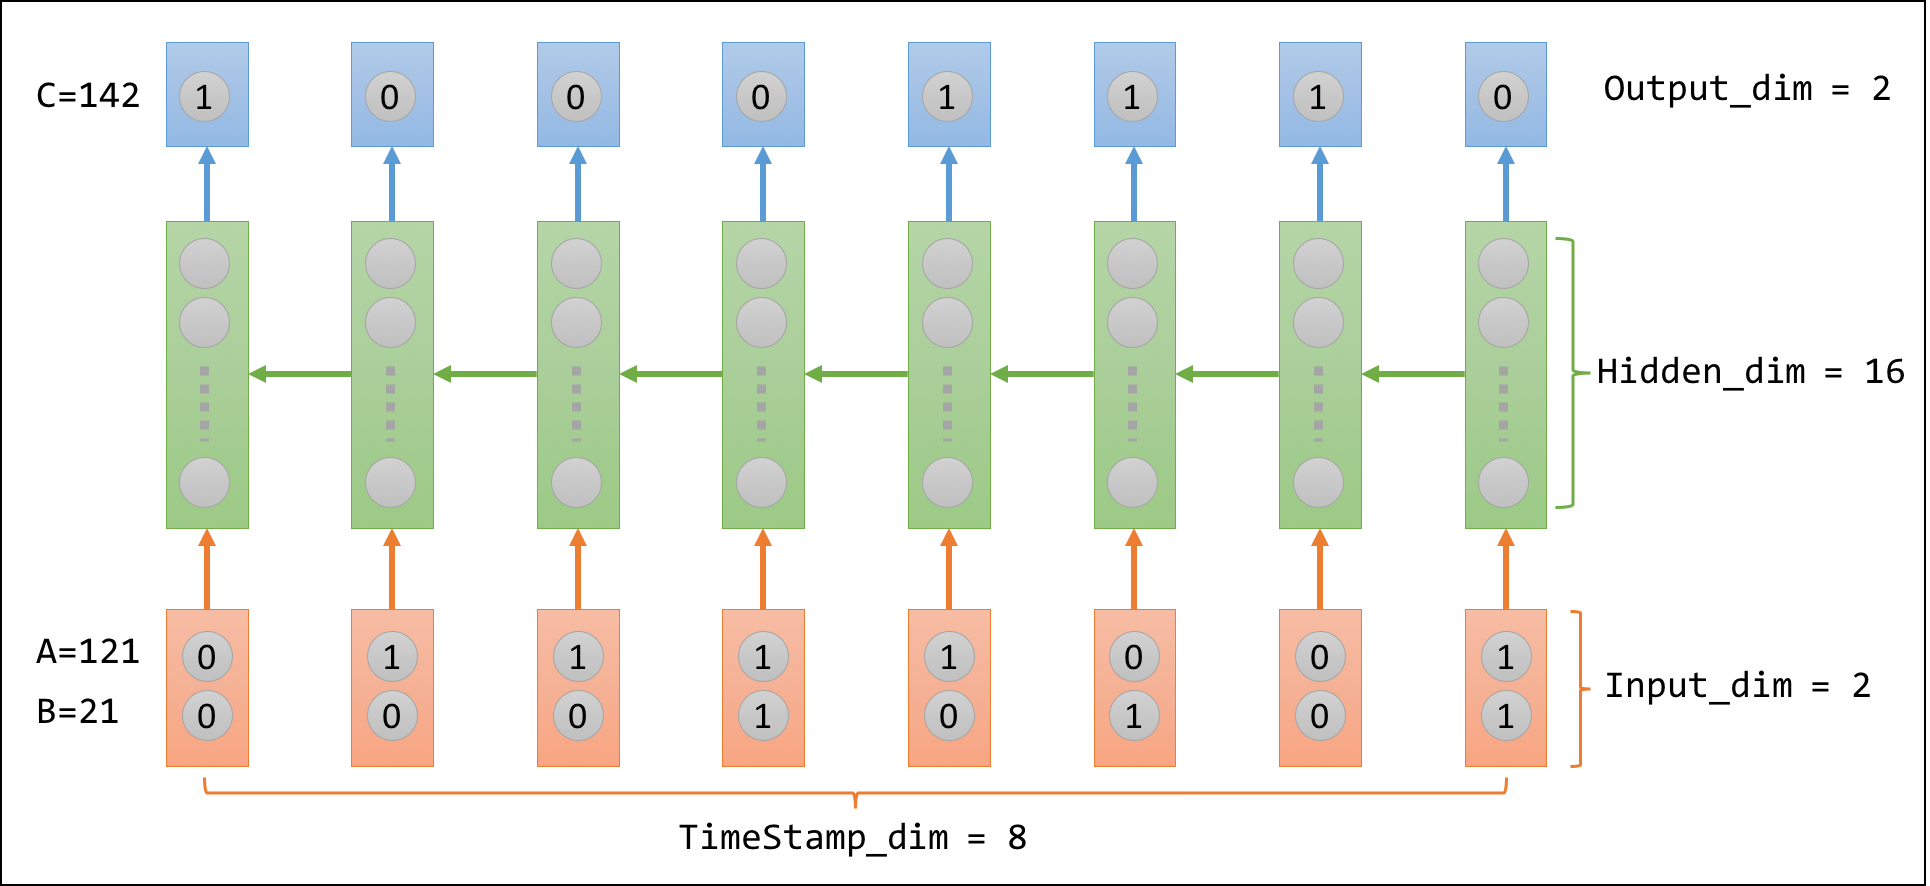
\includegraphics[width=0.8\linewidth]{binary-addition.png}
\caption{Diagram showing proof-of-concept where RNN learns 8 bit binary addition. The green arrows indicating the direction of forward propagation within hidden layer are marked as right-to-left for better illustration of binary addition. R/Rcpp source codes are shared on \href{https://gist.github.com/Puriney/072a37ea8a181f0b6168}{Gist} or shown as in \nameref{appendix} part.}
\label{fig:proof-of-concept}
\end{figure}


Fortunately, model construction is achieved by symbolic configuration in
MXNet. Thus compared with imperative programming (shown as
proof-of-concept above), I have more convenient and feasible approach to
implement advanced models. Things becomes even more easier given that I
have knowledge about the model's topological structure.

The topological structures of variations of RNN are listed below, and
the model listed later depend on the ones stated earlier. Thus my coding
plan is step-by-step, model-by-model, bottom-up.

\subsection{Four types of vanilla RNN}\label{four-types-of-vanilla-rnn}

\begin{figure}[ht]
\centering
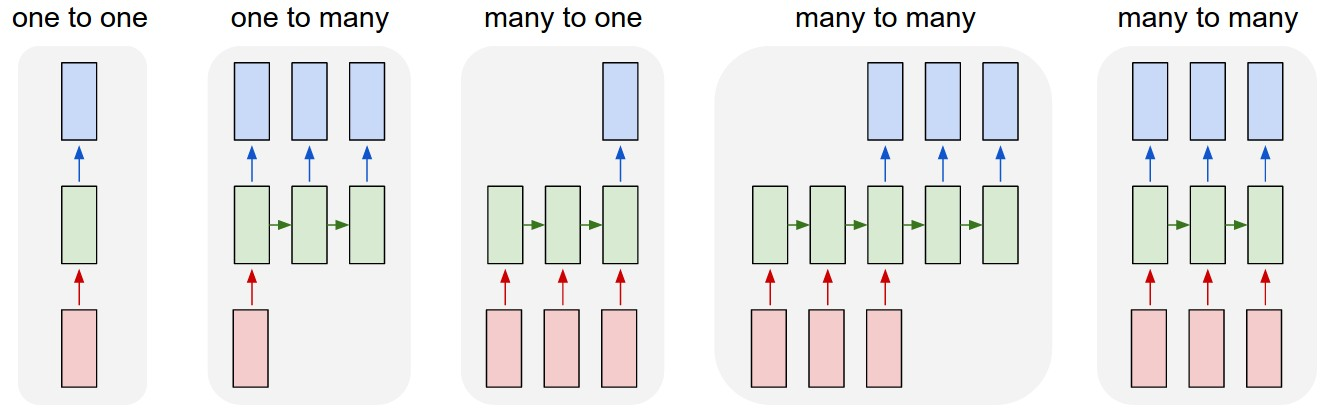
\includegraphics[width=0.8\linewidth]{diags.jpeg}
\caption{Diagram showing basic types of RNN. Red,
green, blue blocks indicate input layer, hidden layer, output layer. And
input/output layer has optional time stamp settings. Source: \href{http://karpathy.github.io/2015/05/21/rnn-effectiveness/}{The Unreasonable Effectiveness of Recurrent Neural Networks}.}
\label{fig:rnn-types}
\end{figure}

The expected snippet of calling vanilla RNN is below:

\begin{Shaded}
\begin{Highlighting}[]
\KeywordTok{mx.symbol.vanillaRNN}\NormalTok{(symbol, name, hidden_dim, }\DataTypeTok{type =} \KeywordTok{c}\NormalTok{(}\StringTok{'1toN'}\NormalTok{, }\StringTok{'Nto1'}\NormalTok{, }\StringTok{'NtoN'}\NormalTok{, }\StringTok{'syncNtoN'}\NormalTok{), ...)}
\end{Highlighting}
\end{Shaded}

My proof-of-concept is imperative programming while the network in built
by symbolic configuration in MXNet. Therefore I plan to implement
high-level API for synced many-to-many RNN at first.

Once imperative-to-declarative translation were finished, solutions for
composing graph of the rest three categories of RNN are expected to be
straightforward, in light of the fact that these three are derivations
of synced many-to-many RNN, shown as Fig-\ref{fig:rnn-opt} .

\begin{figure}[ht]
\centering
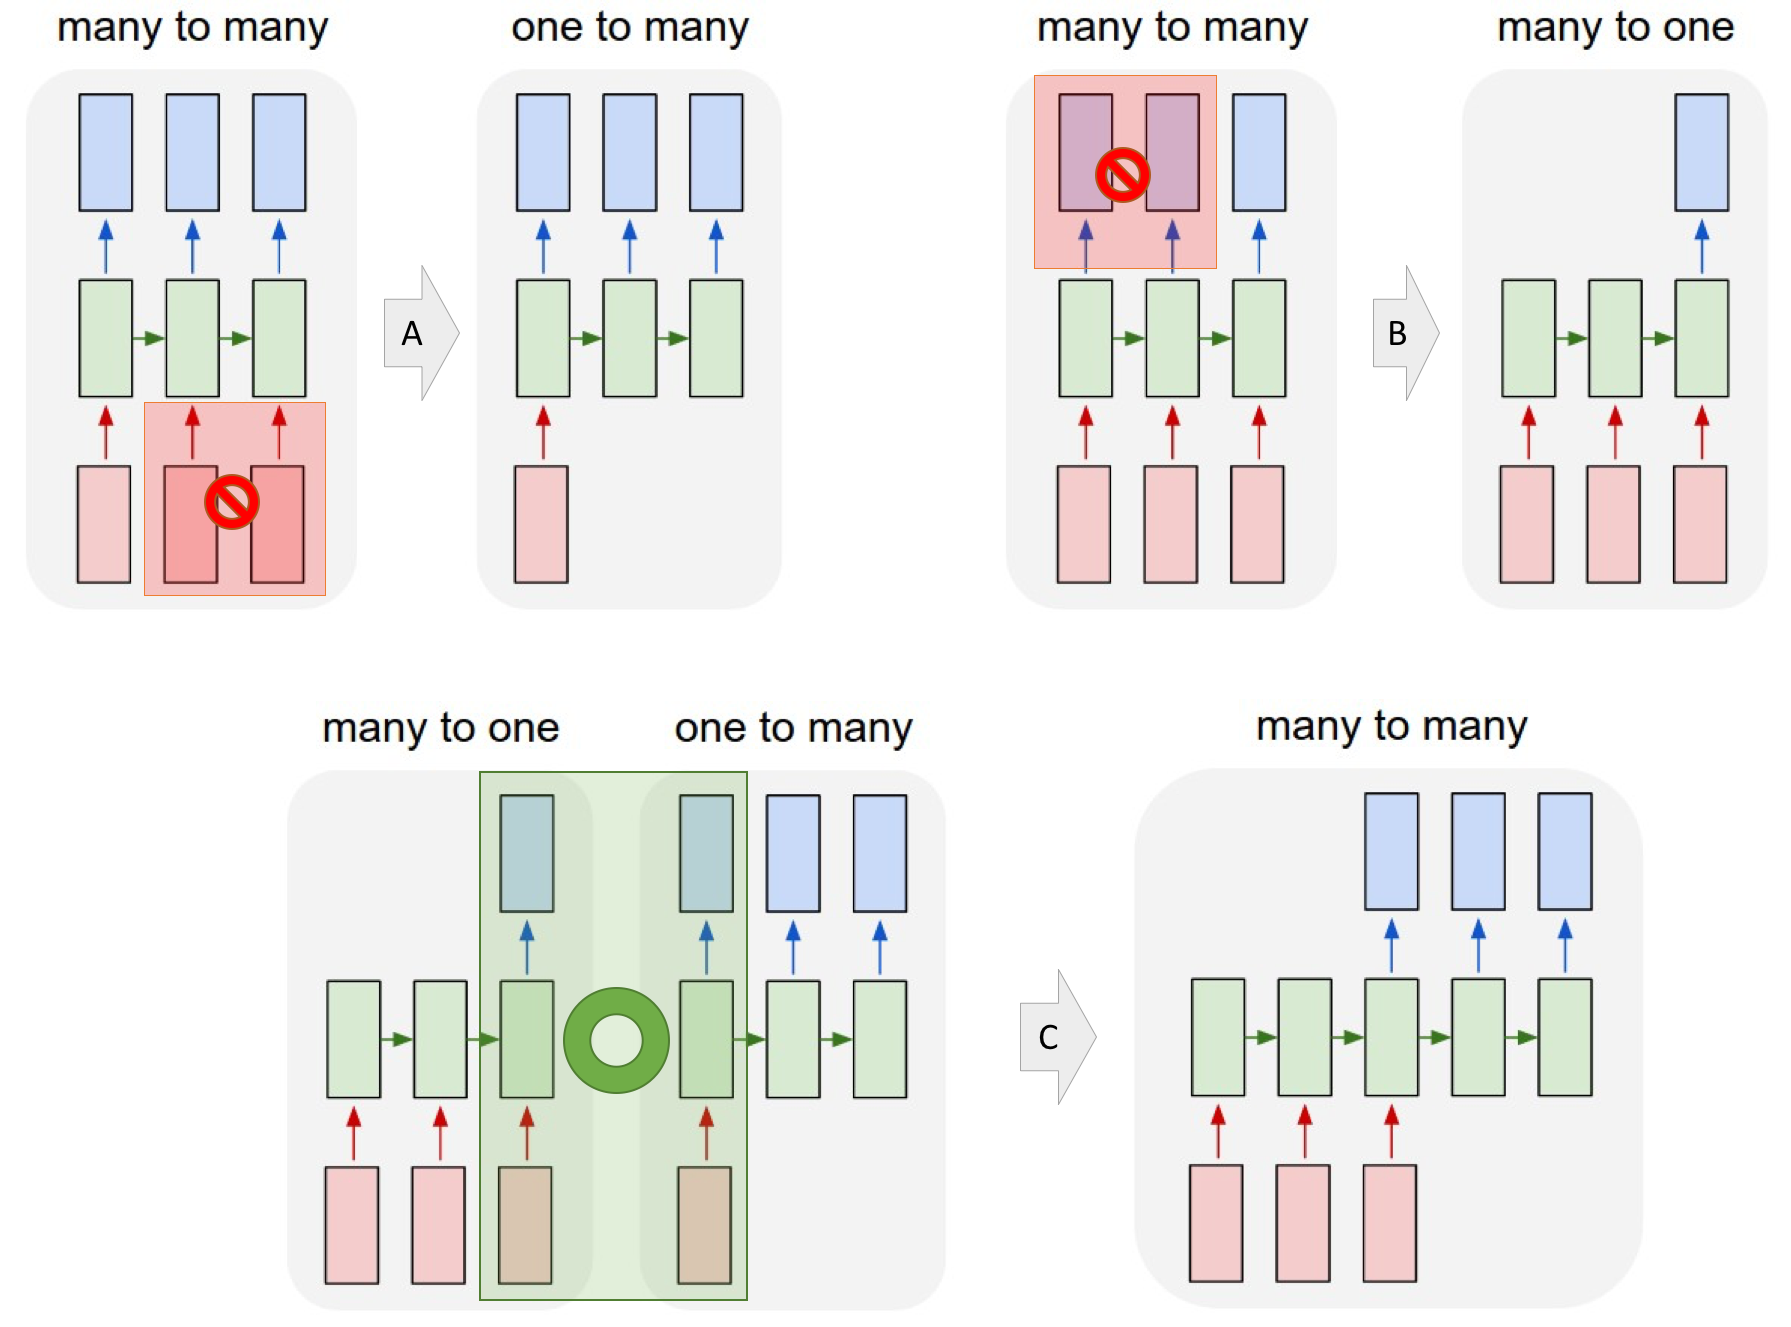
\includegraphics[width=0.7\linewidth]{rnn-models.png}
\caption{Operation A: suppress part of input; Operation B: suppress part of output; Operation C: combine/group the two layers highlighted in green rectangular. Figures are modified from \href{http://karpathy.github.io/2015/05/21/rnn-effectiveness/}{original figure}}
\label{fig:rnn-opt}
\end{figure}

\subsection{LSTM}\label{lstm}

LSTM is specific type of RNN, while it is independently listed given its
popularity.

It has 3 types of gate layers to control the data flow within layers:
forgot, input, and output gate layers.

\begin{figure}[ht]
\centering
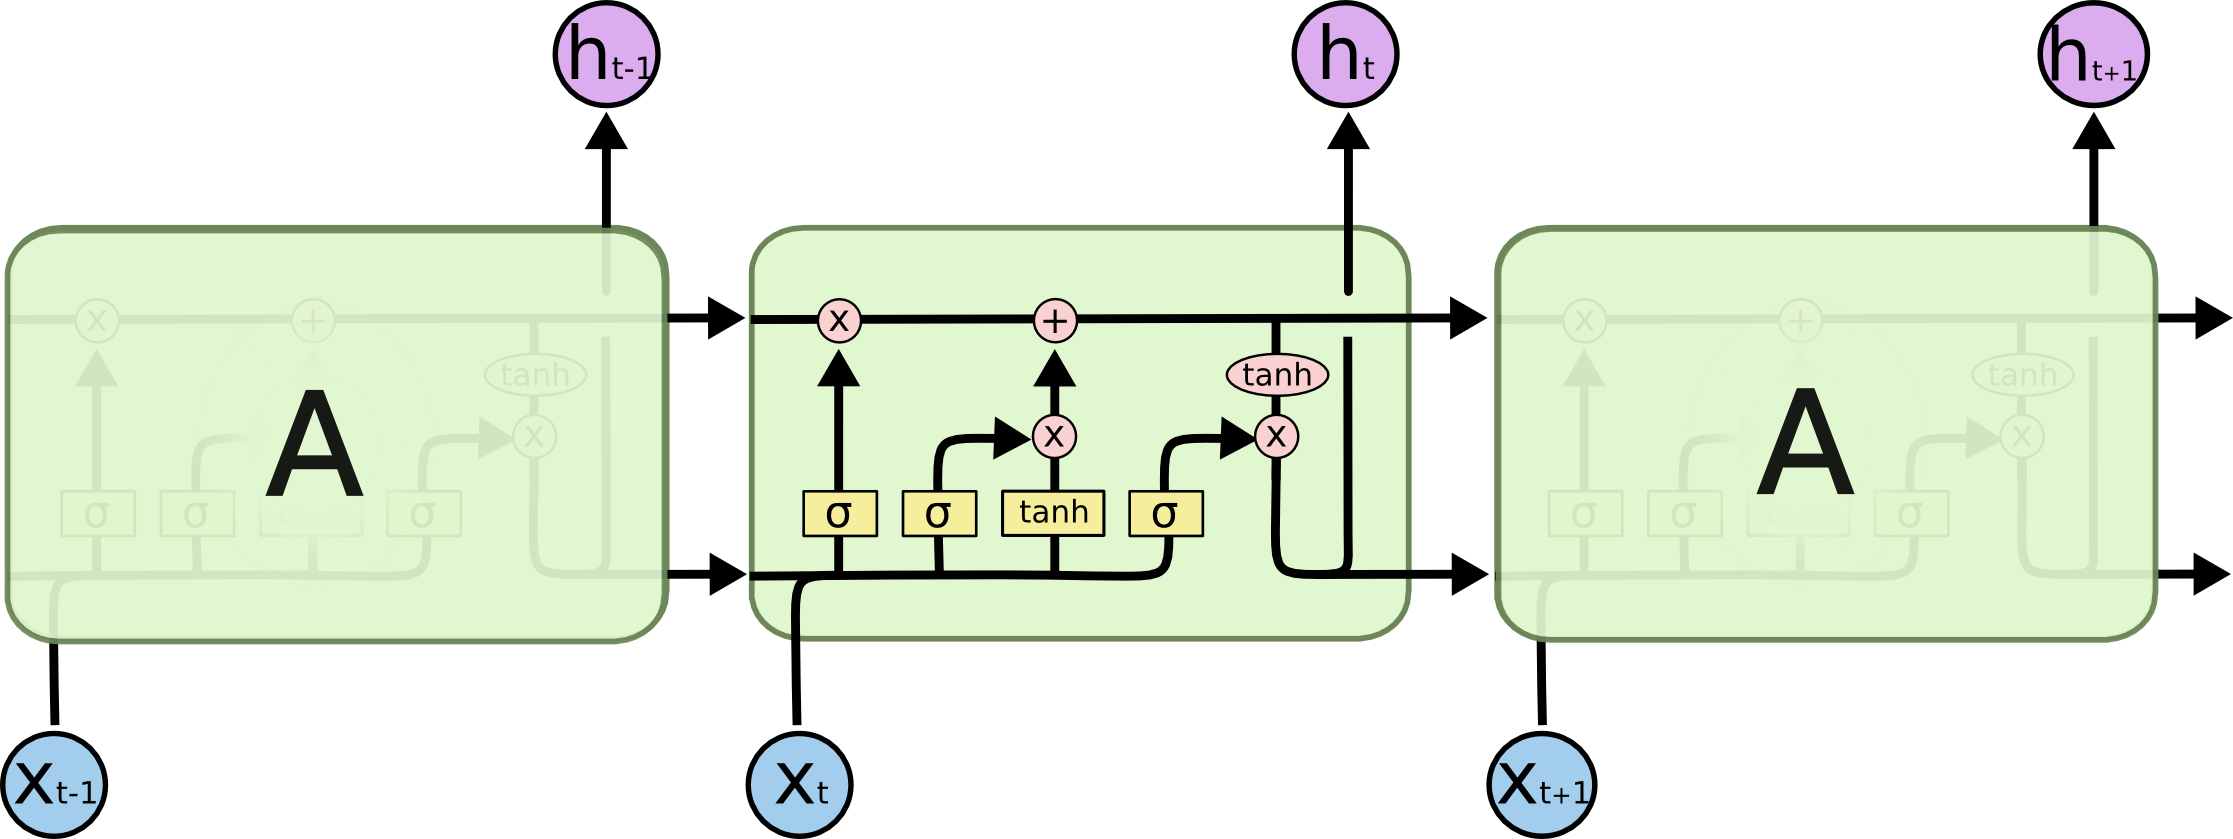
\includegraphics[width=0.7\linewidth]{LSTM3-chain.png}
\caption{The underlying structure of LSTM. Source: \href{http://colah.github.io/posts/2015-08-Understanding-LSTMs/}{Understanding LSTM Networks}}
\label{fig:lstm-3-chain}
\end{figure}


The developer of MXNet's Julia package once posted a step-by-step
\href{http://mxnetjl.readthedocs.org/en/latest/tutorial/char-lstm.html}{tutorial}
for constructing LSTM, in addition to established MXNet's python demos
for LSTM. Therefore I am expected to follow the logics to implement
symbol operation for LSTM. Implementation for LSTM API is expected to be
easiest task throughout this project.

\subsection{GRU}\label{gru}

GRU is derivation of LSTM. It combines input gate and forget gate
combined as update gate, and comes up with other minor modifications, shown as Fig-\ref{fig:gru}.

\begin{figure}[ht]
\centering
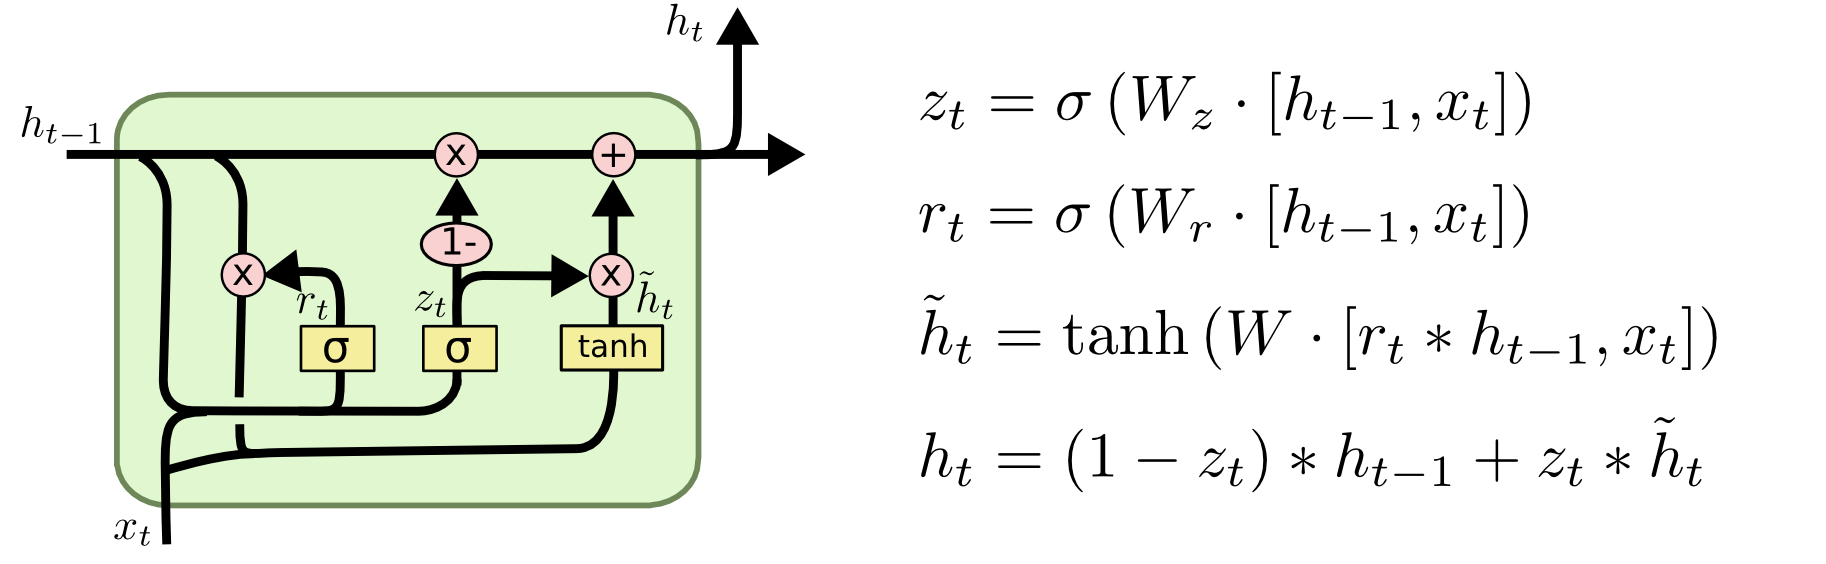
\includegraphics[width=0.7\linewidth]{LSTM3-var-GRU.png}
\caption{Diagram illustrating underlying structure of GRU. Source: \href{http://colah.github.io/posts/2015-08-Understanding-LSTMs/}{Understanding LSTM Networks}}
\label{fig:gru}
\end{figure}

Following the LSTM implementation, GRU is straightforward.

\subsection{Bidirectional RNN}\label{bidirectional-rnn}

Within this computation graph, forward propagation and backward
propagation run through their own layer.

Ref: \href{http://www.cs.toronto.edu/~graves/asru_2013.pdf}{Hybrid
Speech Recognition with. Deep Bidirectional LSTM}

\subsection{Multi-layer RNN}\label{multi-layer-rnn}

RNNs are stacked. Self-explaining (See Fig-\ref{fig:tensorflow} .

\begin{figure}[ht]
\centering
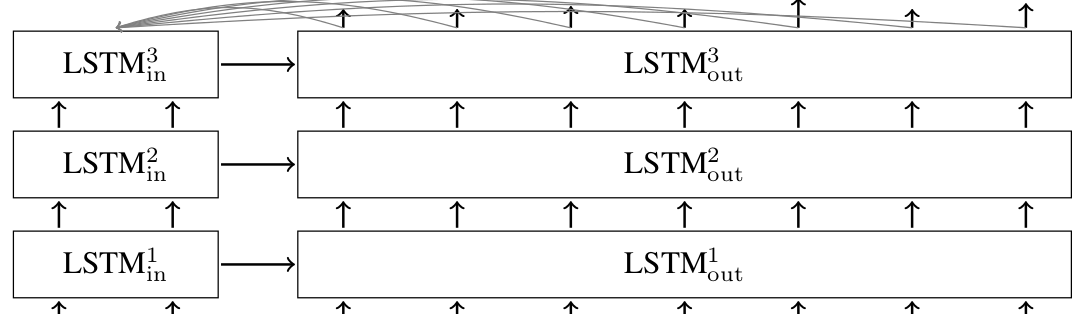
\includegraphics[width=0.8\linewidth]{attention_seq2seq.png}
\caption{Stacked LSTM for attention-based seq2seq model. See \href{https://www.tensorflow.org/versions/r0.7/tutorials/seq2seq/index.html}{source post of TensorFlow}}
\label{fig:tensorflow}
\end{figure}


\subsection{Application in computational
biology}\label{application-in-computational-biology}

I would like to reproduce the CNN model published on Nature magazine in
order to draw attention of R users in bioinformatics, computational
biology field. The results of this possible extra work can also be
checked whether valid by mentors as Qiang Kou had experience in
bioinformatics.

\begin{figure}[ht]
\centering
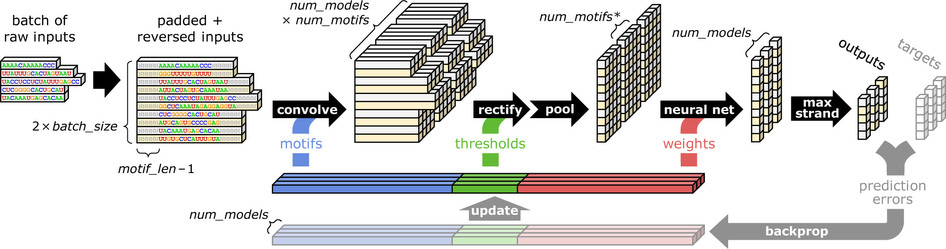
\includegraphics[width=0.8\linewidth]{nbt-cnn.jpg}
\caption{Source:
\href{http://www.nature.com/nbt/journal/v33/n8/full/nbt.3300.html}{Predicting
the sequence specificities of DNA- and RNA-binding proteins by deep
learning}}
\label{fig:10-}
\end{figure}

\section{PERCEIVED OBSTACLES}\label{perceived-obstacles}

The critical turn-overs are:

\begin{enumerate}
\def\labelenumi{\arabic{enumi}.}
\tightlist
\item
  How to precisely adapt my knowledge and existed imperative
  implementation (as the proof-of-concept mentioned before) to MXNet's
  high-level APIs, so that R users could enjoy symbolic configuration.
\item
  How to make APIs support performance as much as possible.
\end{enumerate}

For first part, I could wrap up all basic interfaces to write functions
with parameters to support user-defined network structures, which is the
actual implementation strategy of \texttt{mx.mlp()} layer function for
multilayer perceptron.

If necessary, I would make modifications for \emph{R/src/symbol.cc} etc
to meet development needs. For example, MXNet's develop modified
\emph{symbol.cc} to solve issue reported
\href{https://github.com/dmlc/mxnet/issues/837\#issuecomment-166937031}{here}
which asked for channel slicing to build LSTM.

In addition, basic interfaces contain parameters related to GPU, wrapper
function could take care of performance.

Therefore wrapper-function is going to be qualified and feasible
strategy.

For second part which is native implementation, fortunately MXNet team
maintains a well-documented guide for new developers, in particular the
following posts stated the rules and conventions I need to follow:

\begin{enumerate}
\def\labelenumi{\arabic{enumi}.}
\tightlist
\item
  \href{http://mxnet.readthedocs.org/en/latest/tutorial/new_op_howto.html}{How
  to Create New Operations (Layers)}
\item
  \href{https://mxnet.readthedocs.org/en/latest/developer-guide/operator.html}{Operators
  in MXNet}
\end{enumerate}

For example, the implementation of CNN layer is via three source files
located at directory \emph{src/operator/} : \texttt{convolution-inl.h},
\texttt{convolution.cc}, \texttt{convolution.cu}. In the similar way, I
could implement the new operators for RNN, if necessary. Furthermore,
MXNet's R package has already set up the fundamental interfaces thus my
work will not start from scratch.

Putting things together, I could have feasible approaches to implement
high-level APIs for RNNs and handle perceived problems in affordable
time.

\section{TIMELINE}\label{timeline}

\subsection{Pre-coding period}\label{pre-coding-period}

\rowcolors{1}{white}{gray!10}
\begin{longtable}[l]{ll p{0.7\linewidth}}
\toprule
Start & End & Topic\tabularnewline
\midrule
\endhead
25-Apr-2016 & 1-May-2016 & Read documents. Get familiar with
\textbf{details} of code structure for neural network
symbol.\tabularnewline
2-May-2016 & 8-May-2016 & Read documents. Get familiar with
\textbf{details} of code structure of tensor computation in mxnet so
that I could better adapt my RNN codes for appropriate forward/backward
propagation.\tabularnewline
9-May-2016 & 16-May-2016 & NYU Final exam season.\tabularnewline
17-May-2016 & 22-May-2016 & Contact with mentors to get started. Set up
formal communication tools e.g.~Gitter.\tabularnewline
\bottomrule
\end{longtable}

\subsection{Coding Period}\label{coding-period}

The following 4 jobs must be done when working on every API.

\begin{enumerate}
\def\labelenumi{\arabic{enumi}.}
\tightlist
\item
  Implementation of high-level API;
\item
  \textbf{Testing} (see details of codes tests as sections below);
\item
  \textbf{Write demos and case studies};
\item
  Submit codes and discuss with mentors to see whether they are ready to
  be merged into main stream.
\end{enumerate}

\rowcolors{1}{white}{gray!10}
\begin{longtable}[c]{llp{0.3\linewidth}ll}
\toprule
Start & End & APIs & Demo & Days\tabularnewline
\midrule
\endhead
23-May-2016 & 5-Jun-2016 & Synced Many2Many & Binary Addition &
12\tabularnewline
6-Jun-2016 & 16-Jun-2016 & One2Many & Image Classification &
10\tabularnewline
17-Jun-2016 & 26-Jun-2016 & Many2One & Char RNN & 8\tabularnewline
27-Jun-2016 & 5-Jul-2016 & Many2Many & Translation English to French &
8\tabularnewline
6-Jul-2016 & 14-Jul-2016 & Bidirectional & Translation English to French
& 8\tabularnewline
15-Jul-2016 & 24-Jul-2016 & Stacked & Translation English to French &
8\tabularnewline
25-Jul-2016 & 10-Aug-2016 & LSTM and GRU & Char RNN & 15\tabularnewline
\bottomrule
\end{longtable}

%\rowcolors{1}{white}{gray!10}
\begin{longtable}[c]{@{}llp{0.48\linewidth}ll@{}}
\toprule
Start & End & Application & Reference & Days\tabularnewline
\midrule
\endhead
11-Aug-2016 & 21-Aug-2016 & Case Study of computational biology & Nature
Paper & 9\tabularnewline
\bottomrule
\end{longtable}

(\emph{Days} column excludes Sundays)

In sum, during working period I am glad to actively communicate with
mentors to input more qualified codes into MXNet's R package in addition
to works scheduled here, e.g.~more demos and case studies for users,
other APIs not listed here, etc.

\subsection{Post-coding period}\label{post-coding-period}

22-Aug-2016: Wrapping up the entire project. Because project is
finishing API one-by-one, documents and tests are expected to qualified
and final wrapping up will not take too long.

From 23-Aug-2016 to 29-Aug-2016: Final Evaluation.

\section{MANAGEMENT OF CODING
PROJECT}\label{management-of-coding-project}

\subsection{Where are codes deployed}\label{where-are-codes-deployed}

Fork of MXNet's repository: \url{https://github.com/Puriney/mxnet}.

\subsection{How to test codes}\label{how-to-test-codes}

\subsubsection{Travis Test}\label{travis-test}

My codes can directly use the Travis tests currently used by MXNet's
main repository. Once passing, they are always ready to be merged into
main stream.

\subsubsection{Fast Test}\label{fast-test}

As it is R package, I could use the following snippet to test the R
package.

\begin{Shaded}
\begin{Highlighting}[]
\NormalTok{R CMD check --no-examples --no-manual --no-vignettes --no-build-vignettes mxnet_*.tar.gz}
\end{Highlighting}
\end{Shaded}

In addition, thanks to roxygen2, possible conflicts will be reported
when it generates documents for functions.

\subsubsection{Test against real data}\label{test-against-real-data}

Writing case studies and demos for functions are good conventions of
MXNet and I am expected to follow. In MXNet repository, there existed
data of Penn Treebank Project for RNN, thus I could run test by applying
these data on my codes.

\subsection{Expected Commits
Frequency}\label{expected-commits-frequency}

Commits will be pushed in every 2 days. Commits within a working period
(6 days) are squashed as one commit to make history clean and friendly
to be ready to be merged into MXNet's main repository.

Being absent for 10 days suggests I must come across with problems.

\section{TEST}\label{test}

I fixed an issue and the pull request was afterwards \textbf{merged} (See:
\url{https://github.com/dmlc/mxnet/pull/1554}) into MXNet main
repository, thus I was marked as potential student for this project.

It supports following features:

\begin{itemize}
\tightlist
\item
  Xavier strategy to initialize weights
\item
  Clipping gradient (i.e.~fixing calculated gradient within a range)
\item
  Scheduling mini-changes for learning rate value along training
  process.
\end{itemize}

Passing the tests suggest that I am familiar with MXNet's codes
structure and ready to participate in R language project of MXNet in
GSoC-2016 with matched skills.

\section*{Appendices}\label{appendix}

\begin{Shaded}
\begin{Highlighting}[]
\NormalTok{/}\ErrorTok{/}\StringTok{ }
\ErrorTok{//}\StringTok{ }\NormalTok{Yun Yan}
\NormalTok{/}\ErrorTok{/}\StringTok{ }
\ErrorTok{//}\StringTok{ }\NormalTok{[[Rcpp::}\KeywordTok{plugins}\NormalTok{(cpp11)]]}
\CommentTok{#include <bitset>}
\CommentTok{#include <unordered_set>}
\CommentTok{#include <RcppArmadillo.h>}
\NormalTok{/}\ErrorTok{/}\StringTok{ }\NormalTok{[[Rcpp::}\KeywordTok{depends}\NormalTok{(RcppArmadillo)]]}

\NormalTok{/}\ErrorTok{/}\StringTok{ }\CommentTok{#include <RcppEigen.h>}
\ErrorTok{////}\StringTok{ }\NormalTok{[[Rcpp::}\KeywordTok{depends}\NormalTok{(RcppEigen)]]}

\NormalTok{using namespace Rcpp;}
\NormalTok{/}\ErrorTok{/}\StringTok{ }\NormalTok{using namespace Eigen;}
\NormalTok{using namespace arma;}


\NormalTok{/}\ErrorTok{/}\StringTok{ }\NormalTok{Using Rcpp to reproduce }\StringTok{"RNN in python"}

\NormalTok{/}\ErrorTok{/}\StringTok{' Sigmoid function}
\StringTok{//'}
\NormalTok{/}\ErrorTok{/}\StringTok{' @param x A numeric vector.}
\StringTok{//'} \NormalTok{@export}
\NormalTok{/}\ErrorTok{/}\StringTok{ }\NormalTok{[[Rcpp::export]]}
\NormalTok{NumericVector }\KeywordTok{sigmoid}\NormalTok{(NumericVector x) \{}
  \NormalTok{NumericVector ret =}\StringTok{ }\DecValTok{1} \NormalTok{/}\StringTok{ }\NormalTok{(}\DecValTok{1} \NormalTok{+}\StringTok{ }\KeywordTok{exp}\NormalTok{(-}\DecValTok{1} \NormalTok{*}\StringTok{ }\NormalTok{x));}
  \NormalTok{return ret;}
\NormalTok{\}}

\NormalTok{/}\ErrorTok{/}\StringTok{' First derivative of sigmoid function}
\StringTok{//'}
\NormalTok{/}\ErrorTok{/}\StringTok{' @param x A numeric vector.}
\StringTok{//'} \NormalTok{@export}
\NormalTok{/}\ErrorTok{/}\StringTok{ }\NormalTok{[[Rcpp::export]]}
\NormalTok{NumericVector }\KeywordTok{sigmoid_deriv}\NormalTok{(NumericVector x) \{}
  \NormalTok{return x *}\StringTok{ }\NormalTok{(}\DecValTok{1} \NormalTok{-}\StringTok{ }\NormalTok{x);}
\NormalTok{\}}

\NormalTok{/}\ErrorTok{/}\StringTok{ }\NormalTok{[[Rcpp::export]]}
\NormalTok{NumericMatrix }\KeywordTok{dotprodmm}\NormalTok{(NumericMatrix a, NumericMatrix b) \{}
  \NormalTok{/}\ErrorTok{/}\StringTok{ }\NormalTok{dotprod =}\StringTok{ }\NormalTok{matrix %*%}\StringTok{ }\NormalTok{matrix}
  \NormalTok{mat aa =}\StringTok{ }\NormalTok{as<mat>(a);}
  \NormalTok{mat bb =}\StringTok{ }\NormalTok{as<mat>(b);}
  \NormalTok{mat cc =}\StringTok{ }\NormalTok{aa *}\StringTok{ }\NormalTok{bb;}
  \KeywordTok{return}\NormalTok{(}\KeywordTok{wrap}\NormalTok{(cc));}
\NormalTok{\}}

\NormalTok{/}\ErrorTok{/}\StringTok{ }\NormalTok{[[Rcpp::export]]}
\NormalTok{NumericMatrix }\KeywordTok{dotprodvm}\NormalTok{(NumericVector a, NumericMatrix b) \{}
  \NormalTok{/}\ErrorTok{/}\StringTok{ }\NormalTok{dotprod =}\StringTok{ }\NormalTok{vector %*%}\StringTok{ }\NormalTok{matrix}
  \NormalTok{vec a2 =}\StringTok{ }\NormalTok{as<vec>(a); /}\ErrorTok{/}\StringTok{ }\NormalTok{vector to }\DecValTok{1}\NormalTok{-by-n matrix}
  \NormalTok{int n =}\StringTok{ }\KeywordTok{a.size}\NormalTok{();}
  \NormalTok{mat aa;}
  \KeywordTok{aa.insert_cols}\NormalTok{(}\DecValTok{0}\NormalTok{, a2);}
  \KeywordTok{aa.reshape}\NormalTok{(}\DecValTok{1}\NormalTok{, n);}

  \NormalTok{mat bb =}\StringTok{ }\NormalTok{as<mat>(b);}
  \NormalTok{mat cc =}\StringTok{ }\NormalTok{aa *}\StringTok{ }\NormalTok{bb;}
  \KeywordTok{return}\NormalTok{(}\KeywordTok{wrap}\NormalTok{(cc));}
\NormalTok{\}}

\NormalTok{/}\ErrorTok{/}\StringTok{ }\NormalTok{[[Rcpp::export]]}
\NormalTok{NumericVector }\KeywordTok{m2v}\NormalTok{(NumericMatrix x)\{}
  \NormalTok{/}\ErrorTok{/}\StringTok{ }\NormalTok{matrix to n-by}\DecValTok{-1} \NormalTok{pseudo-vector}
  \NormalTok{mat mx =}\StringTok{ }\NormalTok{as<mat>(x);}
  \NormalTok{vec ret =}\StringTok{ }\KeywordTok{vectorise}\NormalTok{(mx);}
  \KeywordTok{return}\NormalTok{(}\KeywordTok{wrap}\NormalTok{(ret));}
\NormalTok{\}}

\NormalTok{/}\ErrorTok{/}\StringTok{ }\NormalTok{[[Rcpp::export]]}
\NormalTok{NumericMatrix }\KeywordTok{v2m}\NormalTok{(NumericVector v, int nrow, int ncol)\{}
  \NormalTok{NumericMatrix }\KeywordTok{out}\NormalTok{(nrow, ncol);}
  \NormalTok{for (int }\DataTypeTok{i =} \DecValTok{0}\NormalTok{; i <}\StringTok{ }\KeywordTok{v.size}\NormalTok{(); i++}\StringTok{ }\NormalTok{)\{}
    \NormalTok{out[i] =}\StringTok{ }\NormalTok{v[i];}
  \NormalTok{\}}
  \NormalTok{return out;}
\NormalTok{\}}

\NormalTok{/}\ErrorTok{/}\StringTok{ }\NormalTok{[[Rcpp::export]]}
\NormalTok{NumericMatrix }\KeywordTok{InitialMatrix}\NormalTok{(int nrow, int ncol, bool }\DataTypeTok{fill =} \NormalTok{false)\{}
  \NormalTok{int n =}\StringTok{ }\NormalTok{nrow *}\StringTok{ }\NormalTok{ncol;}
  \NormalTok{NumericMatrix }\KeywordTok{ret}\NormalTok{(nrow, ncol);}
  \NormalTok{NumericVector::iterator i =}\StringTok{ }\KeywordTok{ret.begin}\NormalTok{();}
  \NormalTok{NumericVector::iterator j;}
  \NormalTok{NumericVector val;}
  \NormalTok{if (fill ==}\StringTok{ }\NormalTok{true) \{}
    \NormalTok{val =}\StringTok{ }\KeywordTok{rep}\NormalTok{(NumericVector::}\KeywordTok{create}\NormalTok{(}\FloatTok{0.1}\NormalTok{), n);}
  \NormalTok{\} else \{}
    \NormalTok{val =}\StringTok{ }\KeywordTok{runif}\NormalTok{(n);}
  \NormalTok{\}}
  \NormalTok{for (}\DataTypeTok{j =} \KeywordTok{val.begin}\NormalTok{(); j !=}\StringTok{ }\KeywordTok{val.end}\NormalTok{(); ++i, ++j) \{}
    \NormalTok{*i =}\StringTok{ }\ErrorTok{*}\NormalTok{j;}
  \NormalTok{\}}
  \NormalTok{return }\KeywordTok{clone}\NormalTok{(ret);}
\NormalTok{\}}

\NormalTok{/}\ErrorTok{/}\StringTok{ }\NormalTok{[[Rcpp::export]]}
\NormalTok{NumericMatrix }\KeywordTok{dotrans}\NormalTok{(NumericMatrix x)\{}
  \NormalTok{mat xx =}\StringTok{ }\NormalTok{as<mat>(x);}
  \KeywordTok{return}\NormalTok{(}\KeywordTok{wrap}\NormalTok{(}\KeywordTok{xx.t}\NormalTok{()));}
\NormalTok{\}}

\NormalTok{/}\ErrorTok{/}\StringTok{ }\NormalTok{[[Rcpp::export]]}
\NormalTok{List }\KeywordTok{RNN_Train}\NormalTok{(NumericVector A, NumericVector B, bool verbose)\{}
  \NormalTok{/}\ErrorTok{/}\StringTok{ }\NormalTok{network basic parameters}
  \NormalTok{double alpha =}\StringTok{ }\FloatTok{0.1}\NormalTok{;}
  \NormalTok{int input_dim =}\StringTok{ }\DecValTok{2}\NormalTok{;}
  \NormalTok{int hidden_dim =}\StringTok{ }\DecValTok{16}\NormalTok{;}
  \NormalTok{int output_dim =}\StringTok{ }\DecValTok{1}\NormalTok{;}
  \NormalTok{int const bin_dim =}\StringTok{ }\DecValTok{8}\NormalTok{;}

  \NormalTok{/}\ErrorTok{/}\StringTok{ }\NormalTok{network weights; [final output]}
  \NormalTok{NumericMatrix syn0 =}\StringTok{ }\DecValTok{2} \NormalTok{*}\StringTok{ }\KeywordTok{InitialMatrix}\NormalTok{(input_dim, hidden_dim) -}\StringTok{ }\DecValTok{1}\NormalTok{;}
  \NormalTok{NumericMatrix syn1 =}\StringTok{ }\DecValTok{2} \NormalTok{*}\StringTok{ }\KeywordTok{InitialMatrix}\NormalTok{(hidden_dim, output_dim) -}\StringTok{ }\DecValTok{1}\NormalTok{;}
  \NormalTok{NumericMatrix synh =}\StringTok{ }\DecValTok{2} \NormalTok{*}\StringTok{ }\KeywordTok{InitialMatrix}\NormalTok{(hidden_dim, hidden_dim) -}\StringTok{ }\DecValTok{1}\NormalTok{;}
\NormalTok{/}\ErrorTok{/}\StringTok{   }\NormalTok{syn0 =}\StringTok{ }\NormalTok{syn0 *}\StringTok{ }\DecValTok{0} \NormalTok{+}\StringTok{ }\FloatTok{0.1}\NormalTok{;}
\NormalTok{/}\ErrorTok{/}\StringTok{   }\NormalTok{syn1 =}\StringTok{ }\NormalTok{syn1 *}\StringTok{ }\DecValTok{0} \NormalTok{+}\StringTok{ }\FloatTok{0.1}\NormalTok{;}
\NormalTok{/}\ErrorTok{/}\StringTok{   }\NormalTok{synh =}\StringTok{ }\NormalTok{synh *}\StringTok{ }\DecValTok{0} \NormalTok{+}\StringTok{ }\FloatTok{0.1}\NormalTok{;}

  \NormalTok{NumericMatrix syn0_up =}\StringTok{ }\KeywordTok{InitialMatrix}\NormalTok{(input_dim, hidden_dim) *}\StringTok{ }\DecValTok{0}\NormalTok{;}
  \NormalTok{NumericMatrix syn1_up =}\StringTok{ }\KeywordTok{InitialMatrix}\NormalTok{(hidden_dim, output_dim) *}\StringTok{ }\DecValTok{0}\NormalTok{;}
  \NormalTok{NumericMatrix synh_up =}\StringTok{ }\KeywordTok{InitialMatrix}\NormalTok{(hidden_dim, hidden_dim) *}\StringTok{ }\DecValTok{0}\NormalTok{;}

  \NormalTok{/}\ErrorTok{/}\StringTok{ }\NormalTok{correct answer}
  \NormalTok{NumericVector C =}\StringTok{ }\NormalTok{A +}\StringTok{ }\NormalTok{B;}

  \NormalTok{int N =}\StringTok{ }\KeywordTok{A.size}\NormalTok{();}
  \NormalTok{for (int }\DataTypeTok{smp_i =} \DecValTok{0}\NormalTok{; smp_i <}\StringTok{ }\NormalTok{N; smp_i ++) \{ /}\ErrorTok{/}\StringTok{ }\NormalTok{iterate each sample}
    \NormalTok{if (verbose) \{}
      \NormalTok{Rcout <}\ErrorTok{<}\StringTok{ "## Sample: "} \NormalTok{<}\ErrorTok{<}\StringTok{ }\NormalTok{smp_i <}\ErrorTok{<}\StringTok{ }\NormalTok{std::endl;}
      \NormalTok{Rcout <}\ErrorTok{<}\StringTok{ "syn0(0,0) = "} \NormalTok{<}\ErrorTok{<}\StringTok{ }\KeywordTok{syn0}\NormalTok{(}\DecValTok{0}\NormalTok{, }\DecValTok{0}\NormalTok{) <}\ErrorTok{<}\StringTok{ }\NormalTok{std::endl;}
    \NormalTok{\}}
    \NormalTok{int aint =}\StringTok{ }\NormalTok{A[smp_i];}
    \NormalTok{int bint =}\StringTok{ }\NormalTok{B[smp_i];}
    \NormalTok{int cint =}\StringTok{ }\NormalTok{C[smp_i];}
    \NormalTok{std::bitset<bin_dim>}\StringTok{ }\KeywordTok{a}\NormalTok{(aint);}
    \NormalTok{std::bitset<bin_dim>}\StringTok{ }\KeywordTok{b}\NormalTok{(bint);}
    \NormalTok{std::bitset<bin_dim>}\StringTok{ }\KeywordTok{c}\NormalTok{(cint);}
    \NormalTok{NumericVector }\KeywordTok{cHat}\NormalTok{(bin_dim); /}\ErrorTok{/}\StringTok{ }\NormalTok{RNN learning binary digit}

    \NormalTok{double err_sum =}\StringTok{ }\FloatTok{0.0}\NormalTok{;}

    \NormalTok{List l2_deltas;}
    \NormalTok{List l1_vals;}
    \KeywordTok{l1_vals.push_back}\NormalTok{(}\KeywordTok{rep}\NormalTok{(NumericVector::}\KeywordTok{create}\NormalTok{(}\DecValTok{0}\NormalTok{), hidden_dim));}

    \NormalTok{/}\ErrorTok{/}\StringTok{ }\NormalTok{FP begins}
    \NormalTok{if (verbose ) Rcout <}\ErrorTok{<}\StringTok{ "-- FP"} \NormalTok{<}\ErrorTok{<}\StringTok{ }\NormalTok{std::endl;}
    \NormalTok{for (std::size_t }\DataTypeTok{i =} \DecValTok{0}\NormalTok{; i <}\StringTok{ }\KeywordTok{a.size}\NormalTok{(); ++i) \{ /}\ErrorTok{/}\StringTok{ }\NormalTok{iterate time-steps}
      \NormalTok{/}\ErrorTok{/}\StringTok{ }\NormalTok{input and output of each time-step}
      \NormalTok{NumericVector x =}\StringTok{ }\NormalTok{NumericVector::}\KeywordTok{create}\NormalTok{(a[i], /}\ErrorTok{/}\StringTok{ }\NormalTok{Notice bit-set operator}
                                              \NormalTok{b[i]); /}\ErrorTok{/}\StringTok{ }\NormalTok{right-most}
      \NormalTok{NumericVector y =}\StringTok{ }\NormalTok{NumericVector::}\KeywordTok{create}\NormalTok{(c[i]);}
      \NormalTok{/}\ErrorTok{/}\StringTok{ }\NormalTok{hidden_layer ~}\StringTok{ }\NormalTok{input +}\StringTok{ }\NormalTok{prev_hidden}
      \NormalTok{NumericVector l1 =}\StringTok{ }\KeywordTok{sigmoid}\NormalTok{(}\KeywordTok{dotprodvm}\NormalTok{(x, syn0) +}
\StringTok{        }\KeywordTok{dotprodvm}\NormalTok{(as<NumericVector>(l1_vals[}\KeywordTok{l1_vals.size}\NormalTok{() -}\StringTok{ }\DecValTok{1}\NormalTok{]), synh));}
                                 
      \NormalTok{/}\ErrorTok{/}\StringTok{ }\NormalTok{output layer}
      \NormalTok{NumericVector l2 =}\StringTok{ }\KeywordTok{sigmoid}\NormalTok{(}\KeywordTok{dotprodvm}\NormalTok{(l1, syn1));}
      \NormalTok{/}\ErrorTok{/}\StringTok{ }\NormalTok{error at output layer}
      \NormalTok{NumericVector l2_err =}\StringTok{ }\NormalTok{y -}\StringTok{ }\NormalTok{l2;}
      \NormalTok{err_sum +}\ErrorTok{=}\StringTok{ }\KeywordTok{sum}\NormalTok{(}\KeywordTok{abs}\NormalTok{(l2_err));}
      \KeywordTok{l2_deltas.push_back}\NormalTok{(l2_err *}\StringTok{ }\KeywordTok{sigmoid_deriv}\NormalTok{(l2));}

      \NormalTok{if (verbose) \{}
        \NormalTok{Rcout <}\ErrorTok{<}\StringTok{ ">> sample "} \NormalTok{<}\ErrorTok{<}\StringTok{ }\NormalTok{smp_i <}\ErrorTok{<}\StringTok{ "pos"} \NormalTok{<}\ErrorTok{<}\StringTok{ }\NormalTok{i <}\ErrorTok{<}\StringTok{ "="} \NormalTok{<}\ErrorTok{<}\StringTok{ }\NormalTok{x <}\ErrorTok{<}\StringTok{ }\NormalTok{std::endl;}
        \NormalTok{Rcout <}\ErrorTok{<}\StringTok{ }\NormalTok{a[bin_dim -}\StringTok{ }\NormalTok{i -}\StringTok{ }\DecValTok{1}\NormalTok{] <}\ErrorTok{<}\StringTok{ }\NormalTok{std::endl;}
        \NormalTok{Rcout <}\ErrorTok{<}\StringTok{ }\NormalTok{l2_err <}\ErrorTok{<}\StringTok{ }\NormalTok{std::endl;}
      \NormalTok{\}}

      \NormalTok{/}\ErrorTok{/}\StringTok{ }\NormalTok{save output to be displayed}
      \NormalTok{cHat[bin_dim -i -}\DecValTok{1}\NormalTok{] =}\StringTok{ }\KeywordTok{round}\NormalTok{(l2[}\DecValTok{0}\NormalTok{]);}
      \NormalTok{/}\ErrorTok{/}\StringTok{ }\NormalTok{save hidden layer to be used for next time-step}
      \KeywordTok{l1_vals.push_back}\NormalTok{(}\KeywordTok{clone}\NormalTok{(l1));}
    \NormalTok{\}}
    \NormalTok{/}\ErrorTok{/}\StringTok{ }\NormalTok{FP ends}

    \NormalTok{if (verbose) \{}
      \NormalTok{for (List::iterator }\DataTypeTok{li =} \KeywordTok{l1_vals.begin}\NormalTok{(); li !=}\StringTok{ }\KeywordTok{l1_vals.end}\NormalTok{(); li ++)\{}
        \NormalTok{Rcout <}\ErrorTok{<}\StringTok{ "l1 vals: "} \NormalTok{<}\ErrorTok{<}\StringTok{ }\NormalTok{as<NumericVector>(*li) <}\ErrorTok{<}\StringTok{ }\NormalTok{std::endl;}
      \NormalTok{\}}
    \NormalTok{\}}

    \NormalTok{/}\ErrorTok{/}\StringTok{ }\NormalTok{BP begins}
    \NormalTok{if (verbose) Rcout <}\ErrorTok{<}\StringTok{ "-- BP"} \NormalTok{<}\ErrorTok{<}\StringTok{ }\NormalTok{std::endl;}
    \NormalTok{/}\ErrorTok{/}\StringTok{ }\NormalTok{layer}\DecValTok{-1} \NormalTok{at }\StringTok{"next-time"}\NormalTok{-step}
    \NormalTok{NumericVector future_l1_delta =}\StringTok{ }\KeywordTok{rep}\NormalTok{(NumericVector::}\KeywordTok{create}\NormalTok{(}\DecValTok{0}\NormalTok{), hidden_dim);}
    \NormalTok{for (std::size_t }\DataTypeTok{i =} \DecValTok{0}\NormalTok{; i <}\StringTok{ }\KeywordTok{a.size}\NormalTok{(); ++i) \{}
      \NormalTok{NumericVector x =}\StringTok{ }\NormalTok{NumericVector::}\KeywordTok{create}\NormalTok{(a[bin_dim -}\StringTok{ }\NormalTok{i -}\StringTok{ }\DecValTok{1}\NormalTok{],}
                                              \NormalTok{b[bin_dim -}\StringTok{ }\NormalTok{i -}\StringTok{ }\DecValTok{1}\NormalTok{]);}
      \NormalTok{NumericVector l1 =}\StringTok{ }\NormalTok{l1_vals[}\KeywordTok{l1_vals.size}\NormalTok{() -}\StringTok{ }\NormalTok{i -}\StringTok{ }\DecValTok{1}\NormalTok{];}
      \NormalTok{NumericVector l1_prev =}\StringTok{ }\NormalTok{l1_vals[}\KeywordTok{l1_vals.size}\NormalTok{() -}\StringTok{ }\NormalTok{i -}\DecValTok{2}\NormalTok{];}
      \NormalTok{/}\ErrorTok{/}\StringTok{ }\NormalTok{delta at output layer}
      \NormalTok{NumericVector l2_delta =}\StringTok{ }\NormalTok{l2_deltas[}\KeywordTok{l2_deltas.size}\NormalTok{() -i -}\StringTok{ }\DecValTok{1}\NormalTok{];}
      \NormalTok{/}\ErrorTok{/}\StringTok{ }\NormalTok{delta at hidden layer}
      \NormalTok{NumericVector l1_delta =}\StringTok{ }\NormalTok{(}\KeywordTok{dotprodvm}\NormalTok{(l2_delta, }\KeywordTok{dotrans}\NormalTok{(syn1)) +}
\StringTok{                               }\KeywordTok{dotprodvm}\NormalTok{(future_l1_delta, }\KeywordTok{dotrans}\NormalTok{(synh))) *}
\StringTok{                               }\KeywordTok{sigmoid_deriv}\NormalTok{(l1);}
      \NormalTok{/}\ErrorTok{/}\StringTok{ }\NormalTok{collect updates untill all time-steps finished}
      \NormalTok{syn1_up +}\ErrorTok{=}\StringTok{ }\KeywordTok{dotprodmm}\NormalTok{(}\KeywordTok{v2m}\NormalTok{(l1, }\KeywordTok{l1.size}\NormalTok{(), }\DecValTok{1}\NormalTok{),}
                           \KeywordTok{v2m}\NormalTok{(l2_delta, }\DecValTok{1}\NormalTok{, }\KeywordTok{l2_delta.size}\NormalTok{()));}
      \NormalTok{synh_up +}\ErrorTok{=}\StringTok{ }\KeywordTok{dotprodmm}\NormalTok{(}\KeywordTok{v2m}\NormalTok{(l1_prev, }\KeywordTok{l1_prev.size}\NormalTok{(), }\DecValTok{1}\NormalTok{),}
                           \KeywordTok{v2m}\NormalTok{(l1_delta, }\DecValTok{1}\NormalTok{, }\KeywordTok{l1_delta.size}\NormalTok{()));}
      \NormalTok{syn0_up +}\ErrorTok{=}\StringTok{ }\KeywordTok{dotprodmm}\NormalTok{(}\KeywordTok{v2m}\NormalTok{(x, }\KeywordTok{x.size}\NormalTok{(), }\DecValTok{1}\NormalTok{),}
                           \KeywordTok{v2m}\NormalTok{(l1_delta, }\DecValTok{1}\NormalTok{, }\KeywordTok{l1_delta.size}\NormalTok{()));}

      \NormalTok{future_l1_delta =}\StringTok{ }\NormalTok{l1_delta;}

      \NormalTok{if (verbose)\{}
        \NormalTok{Rcout <}\ErrorTok{<}\StringTok{ "bp input at pos: "} \NormalTok{<}\ErrorTok{<}\StringTok{ }\NormalTok{i <}\ErrorTok{<}\StringTok{ "="} \NormalTok{<}\ErrorTok{<}\StringTok{ }\NormalTok{x <}\ErrorTok{<}\StringTok{ }\NormalTok{std::endl;}
        \NormalTok{Rcout <}\ErrorTok{<}\StringTok{ "future delta: "} \NormalTok{<}\ErrorTok{<}\StringTok{ }\NormalTok{future_l1_delta <}\ErrorTok{<}\StringTok{ }\NormalTok{std::endl;}
      \NormalTok{\}}
    \NormalTok{\}}
    \NormalTok{/}\ErrorTok{/}\StringTok{ }\NormalTok{BP ends here}

    \NormalTok{/}\ErrorTok{/}\StringTok{ }\NormalTok{Update netowrk parameters}
    \NormalTok{syn0 +}\ErrorTok{=}\StringTok{ }\NormalTok{(syn0_up *}\StringTok{ }\NormalTok{alpha);}
    \NormalTok{syn1 +}\ErrorTok{=}\StringTok{ }\NormalTok{(syn1_up *}\StringTok{ }\NormalTok{alpha);}
    \NormalTok{synh +}\ErrorTok{=}\StringTok{ }\NormalTok{(synh_up *}\StringTok{ }\NormalTok{alpha);}

    \NormalTok{syn0_up =}\StringTok{ }\KeywordTok{InitialMatrix}\NormalTok{(input_dim, hidden_dim) *}\StringTok{ }\DecValTok{0}\NormalTok{;}
    \NormalTok{syn1_up =}\StringTok{ }\KeywordTok{InitialMatrix}\NormalTok{(hidden_dim, output_dim) *}\StringTok{ }\DecValTok{0}\NormalTok{;}
    \NormalTok{synh_up =}\StringTok{ }\KeywordTok{InitialMatrix}\NormalTok{(hidden_dim, hidden_dim) *}\StringTok{ }\DecValTok{0}\NormalTok{;}

    \NormalTok{if (verbose) \{}
      \NormalTok{Rcout <}\ErrorTok{<}\StringTok{ "!!After"} \NormalTok{<}\ErrorTok{<}\StringTok{ }\NormalTok{std::endl;}
      \NormalTok{Rcout <}\ErrorTok{<}\StringTok{ }\KeywordTok{syn0}\NormalTok{(}\DecValTok{0}\NormalTok{, }\DecValTok{0}\NormalTok{) <}\ErrorTok{<}\StringTok{ }\KeywordTok{syn0}\NormalTok{(}\DecValTok{0}\NormalTok{, }\DecValTok{1}\NormalTok{) <}\ErrorTok{<}\StringTok{ }\KeywordTok{syn0}\NormalTok{(}\DecValTok{1}\NormalTok{, }\DecValTok{0}\NormalTok{) <}\ErrorTok{<}\StringTok{ }\KeywordTok{syn0}\NormalTok{(}\DecValTok{1}\NormalTok{, }\DecValTok{1}\NormalTok{) <}\ErrorTok{<}\StringTok{ }\NormalTok{std::endl;}
      \NormalTok{Rcout <}\ErrorTok{<}\StringTok{ }\KeywordTok{syn1}\NormalTok{(}\DecValTok{0}\NormalTok{, }\DecValTok{0}\NormalTok{) <}\ErrorTok{<}\StringTok{ }\KeywordTok{syn1}\NormalTok{(}\DecValTok{1}\NormalTok{, }\DecValTok{0}\NormalTok{) <}\ErrorTok{<}\StringTok{ }\KeywordTok{syn1}\NormalTok{(}\DecValTok{2}\NormalTok{, }\DecValTok{0}\NormalTok{) <}\ErrorTok{<}\StringTok{ }\KeywordTok{syn1}\NormalTok{(}\DecValTok{0}\NormalTok{, }\DecValTok{3}\NormalTok{) <}\ErrorTok{<}\StringTok{ }\NormalTok{std::endl;}
      \NormalTok{Rcout <}\ErrorTok{<}\StringTok{ }\KeywordTok{synh}\NormalTok{(}\DecValTok{0}\NormalTok{, }\DecValTok{0}\NormalTok{) <}\ErrorTok{<}\StringTok{ }\KeywordTok{synh}\NormalTok{(}\DecValTok{0}\NormalTok{, }\DecValTok{1}\NormalTok{) <}\ErrorTok{<}\StringTok{ }\KeywordTok{synh}\NormalTok{(}\DecValTok{1}\NormalTok{, }\DecValTok{0}\NormalTok{) <}\ErrorTok{<}\StringTok{ }\KeywordTok{synh}\NormalTok{(}\DecValTok{1}\NormalTok{, }\DecValTok{1}\NormalTok{) <}\ErrorTok{<}\StringTok{ }\NormalTok{std::endl;}
      \NormalTok{Rcout <}\ErrorTok{<}\StringTok{ }\KeywordTok{syn0_up}\NormalTok{(}\DecValTok{1}\NormalTok{, }\DecValTok{2}\NormalTok{) <}\ErrorTok{<}\StringTok{ }\NormalTok{std::endl;}
    \NormalTok{\}}

    \NormalTok{if (!verbose &&}\StringTok{ }\NormalTok{smp_i % }\DecValTok{1000} \NormalTok{==}\StringTok{ }\DecValTok{0} \NormalTok{)\{}
      \NormalTok{Rcout <}\ErrorTok{<}\StringTok{ "Sample "} \NormalTok{<}\ErrorTok{<}\StringTok{ }\NormalTok{smp_i <}\ErrorTok{<}\StringTok{ }\NormalTok{std::endl;}
      \NormalTok{Rcout <}\ErrorTok{<}\StringTok{ "Overall Error: "} \NormalTok{<}\ErrorTok{<}\StringTok{ }\NormalTok{err_sum <}\ErrorTok{<}\StringTok{ }\NormalTok{std::endl;}
      \NormalTok{Rcout <}\ErrorTok{<}\StringTok{ "Pred: ["} \NormalTok{<}\ErrorTok{<}\StringTok{ }\NormalTok{cHat <}\ErrorTok{<}\StringTok{ "]"} \NormalTok{<}\ErrorTok{<}\StringTok{ }\NormalTok{std::endl;}
      \NormalTok{Rcout <}\ErrorTok{<}\StringTok{ "True: "} \NormalTok{<}\ErrorTok{<}\StringTok{ }\KeywordTok{c.to_string}\NormalTok{() <}\ErrorTok{<}\StringTok{ }\NormalTok{std::endl;}
      \NormalTok{double cHatInt =}\StringTok{ }\FloatTok{0.0}\NormalTok{;}
      \NormalTok{for (int }\DataTypeTok{i =} \DecValTok{0}\NormalTok{; i <}\StringTok{ }\KeywordTok{cHat.size}\NormalTok{(); i ++)\{}
        \NormalTok{cHatInt +}\ErrorTok{=}\StringTok{ }\KeywordTok{pow}\NormalTok{(}\FloatTok{2.0}\NormalTok{, }\KeywordTok{cHat.size}\NormalTok{() -}\StringTok{ }\NormalTok{i -}\StringTok{ }\DecValTok{1}\NormalTok{) *}\StringTok{ }\NormalTok{cHat[i];}
      \NormalTok{\}}
      \NormalTok{Rcout <}\ErrorTok{<}\StringTok{ "Calc Binary: "} \NormalTok{<}\ErrorTok{<}\StringTok{ }\NormalTok{std::endl <}\ErrorTok{<}\StringTok{ }\NormalTok{a <}\ErrorTok{<}\StringTok{ }\NormalTok{std::endl <}\ErrorTok{<}\StringTok{ }\NormalTok{b <}\ErrorTok{<}\StringTok{ }\NormalTok{std::endl;}
      \NormalTok{Rcout <}\ErrorTok{<}\StringTok{ "Calc Decimal: "} \NormalTok{<}\ErrorTok{<}\StringTok{ }\NormalTok{aint <}\ErrorTok{<}\StringTok{ "+"} \NormalTok{<}\ErrorTok{<}\StringTok{ }\NormalTok{bint <}\ErrorTok{<}\StringTok{ "="} \NormalTok{<}\ErrorTok{<}\StringTok{ }\NormalTok{cHatInt <}\ErrorTok{<}\StringTok{ }\NormalTok{std::endl;}
      \NormalTok{Rcout <}\ErrorTok{<}\StringTok{ "----"} \NormalTok{<}\ErrorTok{<}\StringTok{ }\NormalTok{std::endl;}
    \NormalTok{\}}

  \NormalTok{\}}

  \NormalTok{List syn =}\StringTok{ }\NormalTok{List::}\KeywordTok{create}\NormalTok{(_[}\StringTok{"syn0"}\NormalTok{] =}\StringTok{ }\NormalTok{syn0,}
                          \NormalTok{_[}\StringTok{"syn1"}\NormalTok{] =}\StringTok{ }\NormalTok{syn1,}
                          \NormalTok{_[}\StringTok{"synh"}\NormalTok{] =}\StringTok{ }\NormalTok{synh);}
  \NormalTok{return syn;}
\NormalTok{\}}

\NormalTok{/}\ErrorTok{***}\StringTok{ }\NormalTok{R}
\KeywordTok{require}\NormalTok{(Rcpp)}
\KeywordTok{require}\NormalTok{(RcppArmadillo)}
\KeywordTok{require}\NormalTok{(RcppEigen)}
\KeywordTok{set.seed}\NormalTok{(}\DecValTok{2016}\NormalTok{)}
\NormalTok{max_num <-}\StringTok{ }\DecValTok{2}\NormalTok{^}\DecValTok{8} \NormalTok{-}\DecValTok{1}
\NormalTok{n <-}\StringTok{ }\DecValTok{10000}
\NormalTok{A <-}\StringTok{ }\KeywordTok{c}\NormalTok{(}\KeywordTok{sample}\NormalTok{(}\DecValTok{1}\NormalTok{:(max_num/}\DecValTok{2}\NormalTok{), n, }\DataTypeTok{replace =} \NormalTok{T), }\DecValTok{1}\NormalTok{)}
\NormalTok{B <-}\StringTok{ }\KeywordTok{c}\NormalTok{(}\KeywordTok{sample}\NormalTok{(}\DecValTok{1}\NormalTok{:(max_num/}\DecValTok{2}\NormalTok{), n, }\DataTypeTok{replace =} \NormalTok{T), }\DecValTok{1}\NormalTok{)}
\NormalTok{vFlag <-}\StringTok{ }\NormalTok{F}
\NormalTok{rnn_fit <-}\StringTok{ }\KeywordTok{RNN_Train}\NormalTok{(A, B, vFlag)}
\NormalTok{*}\ErrorTok{/}
\end{Highlighting}
\end{Shaded}

\end{document}
